\let\negmedspace\undefined
\let\negthickspace\undefined
\documentclass[journal,12pt,onecolumn]{IEEEtran}
\usepackage{cite}
\usepackage{amsmath,amssymb,amsfonts,amsthm}
\usepackage{algorithmic}
\usepackage{graphicx}
\graphicspath{{./figs/}}
\usepackage{textcomp}
\usepackage{xcolor}
\usepackage{txfonts}
\usepackage{listings}
\usepackage{enumitem}
\usepackage{mathtools}
\usepackage{gensymb}
\usepackage{comment}
\usepackage{caption}
\usepackage[breaklinks=true]{hyperref}
\usepackage{tkz-euclide} 
\usepackage{listings}
\usepackage{gvv}                                          
\usepackage{xparse}
\usepackage{color}                                            
\usepackage{array}                                            
\usepackage{longtable}                                       
\usepackage{calc}                                             
\usepackage{multirow}
\usepackage{multicol}
\usepackage{hhline}                                           
\usepackage{ifthen}                                           
\usepackage{lscape}
\usepackage{tabularx}
\usepackage{array}
\usepackage{float}
\newtheorem{theorem}{Theorem}[section]
\newtheorem{problem}{Problem}
\newtheorem{proposition}{Proposition}[section]
\newtheorem{lemma}{Lemma}[section]
\newtheorem{corollary}[theorem]{Corollary}
\newtheorem{example}{Example}[section]
\newtheorem{definition}[problem]{Definition}
\newcommand{\BEQA}{\begin{eqnarray}}
	\newcommand{\EEQA}{\end{eqnarray}}
\newcommand{\define}{\stackrel{\triangle}{=}}
\theoremstyle{remark}
\newtheorem{rem}{Remark}

\newcommand{\ihat}{\mathbf {\hat \imath}}
\newcommand{\jhat}{\mathbf {\hat \jmath}}
\newcommand{\vect}[1]{\mathbf #1}



\title{CH: CHEMICAL ENGINEERING}
\author{EE25BTECH11042 - Nipun Dasari}
\date{   }


\begin{document}
	
	\bibliographystyle{IEEEtran}
	\vspace{3cm}
	
	\maketitle
	\begin{enumerate}
		
		\item The ratio of boys to girls in a class is $7$ to $3$. Among the options below, an acceptable value for the total number of students in the class is:
		
		\hfill{\brak{\text{GATE CH 2021}}}
		
		\begin{enumerate}
			\begin{multicols}{4}
				\item $21$
				\item $37$
				\item $50$
				\item $73$
			\end{multicols}
		\end{enumerate}
		
		\item A polygon is convex if, for every pair of points, P and Q belonging to the polygon, the line segment PQ lies completely inside or on the polygon. Which one of the following is NOT a convex polygon?
		
		\hfill{\brak{\text{GATE CH 2021}}}
		
		\begin{enumerate} 
		\begin{figure}[h!] 
		\item 	
\includegraphics[width = 0.4\columnwidth]{q2a}
		\item 	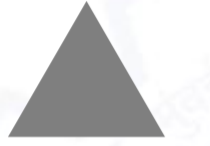
\includegraphics[width = 0.4\columnwidth]{q2b}
		\item	
\includegraphics[width = 0.4\columnwidth]{q2c}
		\item 	
\includegraphics[width = 0.4\columnwidth]{q2d}
			\caption*{}
			\label{fig:q2options}
		\end{figure}
	    \end{enumerate}
		
		\item Consider the following sentences:
		\begin{enumerate}
			\item \brak{i}Everybody in the class is prepared for the exam.
			\item \brak{ii}Babu invited Danish to his home because he enjoys playing chess.
		\end{enumerate}
		Which of the following is the CORRECT observation about the above two sentences?
		
		\hfill{\brak{\text{GATE CH 2021}}}
		
		\begin{enumerate}
			\item \brak{\text{i}} is grammatically correct and \brak{\text{ii}} is unambiguous
			\item \brak{\text{i}} is grammatically incorrect and \brak{\text{ii}} is unambiguous
			\item \brak{\text{i}} is grammatically correct and \brak{\text{ii}} is ambiguous
			\item \brak{\text{i}} is grammatically incorrect and \brak{\text{ii}} is ambiguous
		\end{enumerate}
		
		\item A circular sheet of paper is folded along the lines in the directions shown. The paper, after being punched in the final folded state as shown and unfolded in the reverse order of folding, will look like
		
		\hfill{\brak{\text{GATE CH 2021}}}
		
		\begin{figure}[h!]
			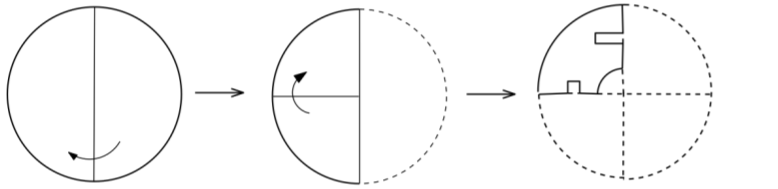
\includegraphics[width = 0.5\columnwidth]{q4}
			\caption*{}
			\label{fig:q4}
		\end{figure}
		
		\begin{enumerate}
			\begin{multicols}{2}
				\item 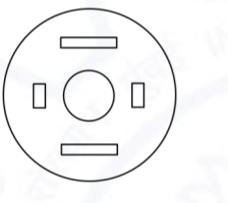
\includegraphics[width = 0.4\columnwidth]{q4a}
				\item 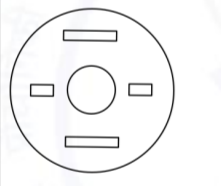
\includegraphics[width = 0.4\columnwidth]{q4b}
				\item 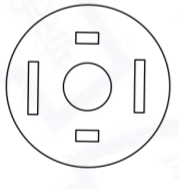
\includegraphics[width = 0.4\columnwidth]{q4c}
				\item 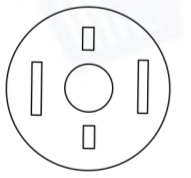
\includegraphics[width = 0.4\columnwidth]{q4d}
			\end{multicols}
		\end{enumerate}
		
		\item \underline{\hspace{2cm}} is to surgery as writer is to \underline{\hspace{2cm}}. Which one of the following options maintains a similar logical relation in the above sentence?
		
		\hfill{\brak{\text{GATE CH 2021}}}
		
		\begin{enumerate}
			\item Plan, outline
			\item Hospital, library
			\item Doctor, book
			\item Medicine, grammar
		\end{enumerate}
		
		\item We have $2$ rectangular sheets of paper, M and N, of dimensions $6~\text{cm} \times 1~\text{cm}$ each. Sheet M is rolled to form an open cylinder by bringing the short edges of the sheet together. Sheet N is cut into equal square patches and assembled to form the largest possible closed cube. Assuming the ends of the cylinder are closed, the ratio of the volume of the cylinder to that of the cube is
		
		\hfill{\brak{\text{GATE CH 2021}}}
		
		\begin{enumerate}
			\begin{multicols}{4}
				\item $\frac{\pi}{2}$
				\item $\frac{3}{\pi}$
				\item $\frac{9}{\pi}$
				\item $3\pi$
			\end{multicols}
		\end{enumerate}
		
		\item Details of prices of two items P and Q are presented in the above table. The ratio of cost of item P to cost of item Q is $3:4$. Discount is calculated as the difference between the marked price and the selling price. The profit percentage is calculated as the ratio of the difference between selling price and cost, to the cost $Profit  = \frac{selling price-cost}{cost} \ times100$. 
		The discount on item Q, as a percentage of its marked price, is
		
		\hfill{\brak{\text{GATE CH 2021}}}
		
		\begin{table}[h!]
			\centering
			\begin{tabular}{|l|l|l|l|}
				\hline
				 items  & cost & profit\% & marked price \\ %do this later
				\hline
				P & $5400$ & ---& $10000$ \\
				\hline
				Q & --- & $25$ & $5860$ \\
				\hline
			\end{tabular}
			\caption*{}
			\label{tab:Q7}
		\end{table}
		
		\begin{enumerate}
			\begin{multicols}{4}
				\item $25$
				\item $12.5$
				\item $10$
				\item $5$
			\end{multicols}
		\end{enumerate}
		
		\item There are five bags each containing identical sets of ten distinct chocolates. One chocolate is picked from each bag. The probability that at least two chocolates are identical is
		
		\hfill{\brak{\text{GATE CH 2021}}}
		
		\begin{enumerate}
			\begin{multicols}{4}
				\item $0.3024$
				\item $0.4235$
				\item $0.6976$
				\item $0.8125$
			\end{multicols}
		\end{enumerate}
		
		\item Given below are two statements $1$ and $2$, and two conclusions I and II.
		\begin{align*}
			\text{Statement 1}&\colon \text{All bacteria are microorganisms.} \\
			\text{Statement 2}&\colon \text{All pathogens are microorganisms.} \\
			\text{Conclusion I}&\colon \text{Some pathogens are bacteria.} \\
			\text{Conclusion II}&\colon \text{All pathogens are not bacteria.}
		\end{align*}
		Based on the above statements and conclusions, which one of the following options is logically CORRECT?
		
		\hfill{\brak{\text{GATE CH 2021}}}
		
		\begin{enumerate}
			\item Only conclusion I is correct
			\item Only conclusion II is correct
			\item Either conclusion I or II is correct.
			\item Neither conclusion I nor II is correct.
		\end{enumerate}
		
		\item Some people suggest anti-obesity measures \brak{\text{AOM}} such as displaying calorie information in restaurant menus. Such measures sidestep addressing the core problems that cause obesity: poverty and income inequality. Which one of the following statements summarizes the passage?
		
		\hfill{\brak{\text{GATE CH 2021}}}
		
		\begin{enumerate}
			\item The proposed AOM addresses the core problems that cause obesity.
			\item If obesity reduces, poverty will naturally reduce, since obesity causes poverty.
			\item AOM are addressing the core problems and are likely to succeed.
			\item AOM are addressing the problem superficially.
		\end{enumerate}
		
		\item An ordinary differential equation \brak{\text{ODE}}, $\frac{dy}{dx}=2y$, with an initial condition $y\brak{0}=1$ has the analytical solution $y=e^{2x}$. Using Runge-Kutta second order method, numerically integrate the ODE to calculate y at $x=0.5$ using a step size of $h=0.5$. If the relative percentage error is defined as, $\epsilon=\abs{\frac{y_{\text{analytical}}-y_{\text{numerical}}}{y_{\text{analytical}}}}\times100$, then the value of $\epsilon$ at $x=0.5$ is
		
		\hfill{\brak{\text{GATE CH 2021}}}
		
		\begin{enumerate}
			\begin{multicols}{4}
				\item $0.06$
				\item $0.8$
				\item $4.0$
				\item $8.0$
			\end{multicols}
		\end{enumerate}
		
		\item The function $\cos\brak{x}$ is approximated using Taylor series around $x=0$ as $\cos\brak{x}\approx1+a~x+b~x^{2}+c~x^{3}+d~x^{4}$. The values of a, b, c and d are
		
		\hfill{\brak{\text{GATE CH 2021}}}
		
		\begin{enumerate}
			\begin{multicols}{2}
			\item $a=1, b=-0.5, c=-1, d=-0.25$
			\item $a=0, b=-0.5, c=0, d=0.042$
			\item $a=0, b=0.5, c=0, d=0.042$
			\item $a=-0.5, b=0, c=0.042, d=0$
		\end{multicols}
		\end{enumerate}
		
		\item A batch settling experiment is performed in a long column using a dilute dispersion containing equal number of particles of type A and type B in water \brak{density= 1000kg/m^{-3}} at room temperature. Type A are spherical particles of diameter $30~\mu\text{m}$ and density $1100kg/m^{-3}$. Type B are spherical particles of diameter $10\mu_{m}$ and density $1900kg/m^{-3}$. Assuming that Stokes' law is valid throughout the duration of the experiment, the settled bed would
		
		\hfill{\brak{\text{GATE CH 2021}}}
		
		\begin{enumerate}
		\item consist of a homogeneous mixture of type A and type B particles
		\item consist of type B particles only
		\item be completely segregated with type B particles on top of type A particles
		\item be completely segregated with type A particles on top of type B particles
		\end{enumerate}
		
		\item The heat of combustion of methane, carbon monoxide and hydrogen are P, Q and R respectively. For the reaction below, $CH_{4}+H_{2}O\longrightarrow CO+3H_{2}$ the heat of reaction is given by
		
		\hfill{\brak{\text{GATE CH 2021}}}
		
		\begin{enumerate}
		\begin{multicols}{4}
			\item $P-Q-3R$
			\item $Q+3R-P$
			\item $P-Q-R$
			\item $Q+R-P$
		\end{multicols}
		\end{enumerate}
		
		\item A three-dimensional velocity field is given by $\myvec{V} = 5x^2y \myvec{i} + Cy \myvec{j} - 10xyz \myvec{k}$, where $\myvec{i}, \myvec{j}, \myvec{k}$ are the unit vectors in $x, y, z$ directions, respectively, describing a cartesian coordinate system. The coefficient $C$ is a constant. If $\myvec{V}$ describes an incompressible fluid flow, the value of $C$ is
		
		\hfill{\brak{\text{GATE CH 2021}}}
		
		\begin{enumerate}
		\begin{multicols}{4}
			\item $-1$
			\item $0$
			\item $1$
			\item $5$
		\end{multicols}
		\end{enumerate}
		
		\item Heat transfer coefficient for a vapor condensing as a film on a vertical surface is given by
		
		\hfill{\brak{\text{GATE CH 2021}}}
		
		\begin{enumerate}
		\item Dittus-Boelter equation
		\item Nusselt theory
		\item Chilton-Colburn analogy
		\item Sieder-Tate equation
		\end{enumerate}
		
		\item In a double-pipe heat exchanger of $10~\text{m}$ length, a hot fluid flows in the annulus and a cold fluid flows in the inner pipe. The temperature profiles of the hot \brak{T_h} and cold \brak{T_c} fluids along the length of the heat exchanger \brak{x \text{such that} x \geq 0}, are given by $T_h\brak{x} = 80 - 3x$ and $T_c\brak{x} = 20 + 2x$, where $T_h$ and $T_c$ are in $\degree\text{C}$, and $x$ is in meter. The logarithmic mean temperature difference \brak{\text{in}} $\degree\text{C}$ is
	
\hfill{\brak{\text{GATE CH 2021}}}

\begin{enumerate}
\begin{multicols}{4}
\item $24.6$
\item $27.9$
\item $30.0$
\item $50.0$
\end{multicols}
\end{enumerate}

\item For a shell-and-tube heat exchanger, the clean overall heat transfer coefficient is calculated as $250~\text{W m}^{-2}\text{ K}^{-1}$ for a specific process condition. It is expected that the heat exchanger may be fouled during the operation, and a fouling resistance of $0.001~\text{m}^{2}\text{ K W}^{-1}$ is prescribed. The dirt overall heat transfer coefficient is \underline{\hspace{2cm}} $\text{W m}^{-2}\text{ K}^{-1}$.

\hfill{\brak{\text{GATE CH 2021}}}

\item In reverse osmosis, the hydraulic pressure and osmotic pressure at the feed side of the membrane are $P_1$ and $\pi_1$, respectively. The corresponding values are $P_2$ and $\pi_2$ at the permeate side. The membrane, feed, and permeate are at the same temperature. For equilibrium to prevail, the general criterion that should be satisfied is

\hfill{\brak{\text{GATE CH 2021}}}

\begin{enumerate}
\begin{multicols}{2}
\item $\pi_1 = \pi_2$
\item $P_1 = P_2$
\item $P_1 + \pi_1 = P_2 + \pi_2$
\item $P_1 - \pi_1 = P_2 - \pi_2$
\end{multicols}
\end{enumerate}

\item Ethylene adsorbs on the vacant active sites $V$ of a transition metal catalyst according to the following mechanism.
\begin{align*}
C_2H_4 + V &\rightleftharpoons C_2H_4 \cdot V \\
C_2H_4 \cdot V + V &\rightleftharpoons C_2H_4 + 2V
\end{align*}
If $N_t$, $N_v$, and $N_{C_2H_4 \cdot V}$ denote the total number of active sites, number of vacant active sites and number of adsorbed $C_2H_4$ molecules, respectively, the balance on the total number of active sites is given by

\hfill{\brak{\text{GATE CH 2021}}}

\begin{enumerate}
\begin{multicols}{2}
\item $N_t = N_v + N_{C_2H_4 \cdot V}$
\item $N_t = N_v - N_{C_2H_4 \cdot V}$
\item $N_t = N_v + 2 N_{C_2H_4 \cdot V}$
\item $N_t = 2 N_v + N_{C_2H_4 \cdot V}$
\end{multicols}
\end{enumerate}

\item Which of the following is NOT a standard to transmit measurement and control signals?

\hfill{\brak{\text{GATE CH 2021}}}

\begin{enumerate}
\begin{multicols}{4}
\item $4-20~\text{mA}$
\item $3-15~\text{psig}$
\item $0-100~\%$
\item $1-5~\text{VDC}$
\end{multicols}
\end{enumerate}

\item A feedforward controller can be used only if

\hfill{\brak{\text{GATE CH 2021}}}

\begin{enumerate}
\item the disturbance variable can be measured
\item the disturbance variable can be manipulated
\item the disturbance variable can be ignored
\item regulatory control is not required
\end{enumerate}

\item Turnover ratio is defined as

\hfill{\brak{\text{GATE CH 2021}}}

\begin{enumerate}
	\begin{multicols}{2}
\item $\frac{\text{Sales}}{\text{Fixed capital}}$
\item $\frac{\text{Sales}}{\text{Working capital}}$
\item $\frac{\text{Working capital}}{\text{Total capital}}$
\item $\frac{\text{Total capital}}{\text{Sales}}$
\end{multicols}
\end{enumerate}

\item A principal amount is charged a nominal annual interest rate of $10\%$. If the interest rate is compounded continuously, the final amount at the end of one year would be

\hfill{\brak{\text{GATE CH 2021}}}

\begin{enumerate}
\item higher than the amount obtained when the interest rate is compounded monthly
\item lower than the amount obtained when the interest rate is compounded annually
\item equal to $1.365$ times the principal amount
\item equal to the amount obtained when using an effective interest rate of $27.18\%$
\end{enumerate}

\item Match the common name of chemicals in Group -- $1$ with their chemical formulae in Group -- $2$.

\hfill{\brak{\text{GATE CH 2021}}}

\begin{table}[h!]
\centering
\begin{tabular}{|l|l|}
\hline
Group -- 1 & Group -- 2 \\
\hline
P Gypsum & I $Ca(H_2PO_4)_2$ \\
\hline
Q Dolomite & II $CaSO_4 \cdot 2H_2O$ \\
\hline
R Triple superphosphate & III $CaCO_3 \cdot MgCO_3$ \\
\hline
\end{tabular}
\caption*{}
\label{tab:Q15}
\end{table}

The correct combination is:
\begin{enumerate}
\begin{multicols}{4}
\item P -- III, Q -- II, R -- I
\item P -- III, Q -- I, R -- II
\item P -- II, Q -- III, R -- I
\item P -- II, Q -- I, R -- III
\end{multicols}
\end{enumerate}

\item For the function $f\brak{x} = \begin{cases} -x, & x < 0 \\ x^2, & x \ge 0 \end{cases}$ the CORRECT statement(s) is/are

\hfill{\brak{\text{GATE CH 2021}}}

\begin{enumerate}
\item $f\brak{x}$ is continuous at $x=1$
\item $f\brak{x}$ is differentiable at $x=1$
\item $f\brak{x}$ is continuous at $x=0$
\item $f\brak{x}$ is differentiable at $x=0$
\end{enumerate}

\item Feed solution F is contacted with solvent B in an extraction process. Carrier liquid in the feed is A and the solute is C. The ternary diagram depicting a single ideal stage extraction is given below. The dashed lines represent the tie-lines.
\begin{figure}[H]
	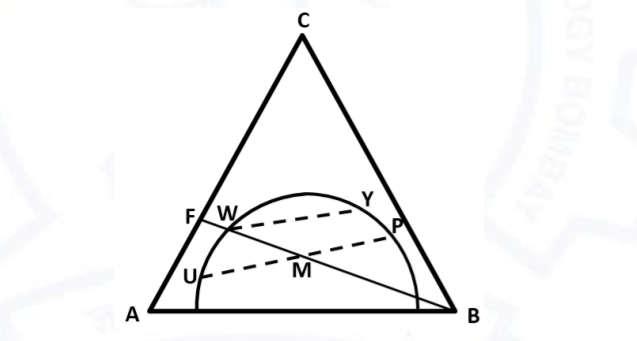
\includegraphics[width = 0.8\columnwidth]{q17.png}
	\caption*{}
	\label{fig:q17}
\end{figure}
 The CORRECT option(s) is/are

\hfill{\brak{\text{GATE CH 2021}}}

\begin{enumerate}
\item For the tie-lines shown, concentration of solute in the extract is higher than that in the raffinate
\item Maximum amount of solvent is required if the mixture composition is at W
\item Y represents the composition of extract when minimum amount of solvent is used
\item U represents the raffinate composition if the mixture composition is at M
\end{enumerate}

\item The inherent characteristics of three control valves P, Q and R are shown in the figure. 
\begin{figure}[H]
	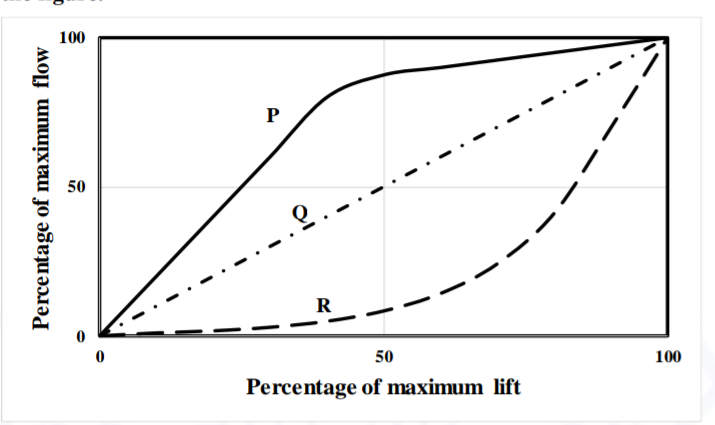
\includegraphics[width = 0.8\columnwidth]{q18.png}
	\caption*{}
	\label{fig:q28}
\end{figure}
The CORRECT option(s) is/are

\hfill{\brak{\text{GATE CH 2021}}}

\begin{enumerate}
\item P is a quick opening valve
\item Q is a quick opening valve
\item P is an equal percentage valve
\item R is an equal percentage valve
\end{enumerate}

\item A source placed at the origin of a circular sample holder \brak{\text{radius} r = 1m} emits particles uniformly in all directions. A detector of length $l = 1cm$ has been placed along the perimeter of the sample holder. During an experiment, the detector registers $14$ particles. The total number of particles emitted during the experiment is \underline{\hspace{2cm}}.

\hfill{\brak{\text{GATE CH 2021}}}

\item $A, B, C$ and $D$ are vectors of length $4$.
\begin{align*}
A &= \myvec{a_1 \\ a_2 \\ a_3 \\ a_4} &
B &= \myvec{b_1 \\ b_2 \\ b_3 \\ b_4} \\
C &= \myvec{c_1 \\ c_2 \\ c_3 \\ c_4} &
D &= \myvec{d_1 \\ d_2 \\ d_3 \\ d_4}
\end{align*}
It is known that $B$ is not a scalar multiple of $A$. Also, $C$ is linearly independent of $A$ and $B$. Further, $D = 3A + 2B + C$. The rank of the matrix $\myvec{a_1 & b_1 & c_1 & d_1 \\ a_2 & b_2 & c_2 & d_2 \\ a_3 & b_3 & c_3 & d_3 \\ a_4 & b_4 & c_4 & d_4}$ is \underline{\hspace{2cm}}.

\hfill{\brak{\text{GATE CH 2021}}}

\item The van der Waals equation of state is given by $P_r = \frac{8T_r}{3v_r - 1} - \frac{3}{v_r^2}$ where $P_r, T_r$ and $v_r$ represent reduced pressure, reduced temperature and reduced molar volume, respectively. The compressibility factor at critical point \brak{z_c} is $3/8$. If $v_r = 3$ and $T_r = 4/3$, then the compressibility factor based on the van der Waals equation of state is \underline{\hspace{2cm}} \brak{\text{round off to 2 decimal places}}.

\hfill{\brak{\text{GATE CH 2021}}}

\item Consider a steady flow of an incompressible, Newtonian fluid through a smooth circular pipe. Let $\alpha_{\text{laminar}}$ and $\alpha_{\text{turbulent}}$ denote the kinetic energy correction factors for laminar and turbulent flow through the pipe, respectively. For turbulent flow through the pipe $\alpha_{\text{turbulent}} = \brak{\frac{V_0}{\bar{V}}}^2 \frac{2n^2 \brak{3+n}}{\brak{3+2n}}$. Here, $\bar{V}$ is the average velocity, $V_0$ is the centerline velocity, and $n$ is a parameter. The ratio of average velocity to the centerline velocity for turbulent flow through the pipe is given by $\frac{\bar{V}}{V_0} = \frac{2n^2}{\brak{n+1}\brak{2n+1}}$. For $n=7$, the value of $\frac{\alpha_{\text{turbulent}}}{\alpha_{\text{laminar}}}$ is \underline{\hspace{2cm}} \brak{\text{round off to 2 decimal places}}.

\hfill{\brak{\text{GATE CH 2021}}}

\item The molar heat capacity at constant pressure $C_p$ \brak{\text{in J mol$^{-1}$ K$^{-1}$}} for n-pentane as a function of temperature \brak{\text{T in K}} is given by $C_p = 100 + 0.21T + 0.0003 T^2$. Take $ r=8.314J/mol^{-1}{K}^{-1}$. At $1000~\text{K}$, the rate of change of molar entropy of n-pentane with respect to temperature at constant pressure is \underline{\hspace{2cm}} $\text{J mol}^{-1}\text{K}^{-2}$ \brak{\text{round off to 2 decimal places}}.

\hfill{\brak{\text{GATE CH 2021}}}

\item The following homogeneous liquid phase reactions are at equilibrium.
\begin{align*}
A + B &\rightleftharpoons C + D & K_1 &= \frac{[C][D]}{[A][B]} = \frac{k_1}{k_{-1}} \\
C + E &\rightleftharpoons F & K_2 &= \frac{[F]}{[C][E]} = \frac{k_2}{k_{-2}} \\
A + B + E &\rightleftharpoons F + D & K_3 &= \frac{[F][D]}{[A][B][E]} = \frac{k_3}{k_{-3}}
\end{align*}
The values of rate constants are given by: $k_1 = 0.1~\text{s}^{-1}, k_{-1} = 0.2~\text{s}^{-1}, k_2 = 1~\text{s}^{-1}, k_{-2} = 10~\text{s}^{-1}, k_3 = 10~\text{s}^{-1}$. The value of rate constant $k_{-3}$ is \underline{\hspace{2cm}} $\text{s}^{-1}$ \brak{\text{round off to 1 decimal place}}.

\hfill{\brak{\text{GATE CH 2021}}}

\item A company invests in a recovery unit to separate valuable metals from effluent streams. The total initial capital investment of this unit is Rs. $10$ lakhs. The recovered metals are worth Rs. $4$ lakhs per year. If the annual return on this investment is $15\%$, the annual operating costs should be \underline{\hspace{2cm}} lakhs of rupees \brak{\text{correct to 1 decimal place}}.


\item Let A be a square matrix of size $n \times n \brak{n > 1}$. The elements of $A = \brak{a_{ij}}$ are given by
\begin{align*}
	a_{ij} = \begin{cases}
		i \times j, & \text{if } i \ge j \\
		0, & \text{if } i < j
	\end{cases}
\end{align*}
The determinant of A is
\hfill{\brak{\text{GATE CH 2021}}}
\begin{enumerate}
	\begin{multicols}{2}
		\item $0$
		\item $1$
		\item $n!$
		\item $\brak{n!}^{2}$
	\end{multicols}
\end{enumerate}

 

\item Consider a fluid confined between two horizontal parallel plates and subjected to shear flow.
In the first experiment, the plates are separated by a distance of $1$ mm. It is found that a shear stress of $2~N~m^{-2}$ has to be applied to keep the top plate moving with a velocity of $2~m~s^{-1}$, while the other plate is fixed.
In the second experiment, the plates are separated by a distance of $0.25$ mm. It is found that a shear stress of $3~N~m^{-2}$ has to be applied to keep the top plate moving with a velocity of $1~m~s^{-1}$, while the other plate is fixed. In the range of shear rates studied, the rheological character of the fluid is
\hfill{\brak{\text{GATE CH 2021}}}
\begin{enumerate}
	\begin{multicols}{2}
		\item Newtonian
		\item Pseudoplastic
		\item Dilatant
		\item Ideal and inviscid
	\end{multicols}
\end{enumerate}

 

\item Water of density $1000$ kg $m^{-3}$ flows in a horizontal pipe of $10$ cm diameter at an average velocity of $0.5~m~s^{-1}$. The following plot shows the pressure measured at various distances from the pipe entrance.
\begin{figure}[H]
	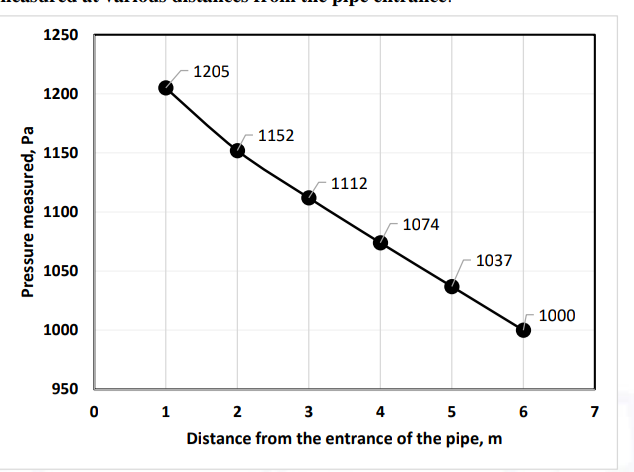
\includegraphics[width = 0.8\columnwidth]{q28.png}
	\caption*{}
	\label{fig:q28}
\end{figure}
Using the data shown in the figure, the Fanning friction factor in the pipe when the flow is FULLY DEVELOPED is
\hfill{\brak{\text{GATE CH 2021}}}
\begin{enumerate}
	\begin{multicols}{2}
		\item $0.0012$
		\item $0.0074$
		\item $0.0082$
		\item $0.0106$
	\end{multicols}
\end{enumerate}

 

\item In a solvent regeneration process, a gas is used to strip a solute from a liquid in a countercurrent packed tower operating under isothermal condition. Pure gas is used in this stripping operation. All solutions are dilute and Henry's law, $y^{*}=mx$, is applicable. Here, $y^{*}$ is the mole fraction of the solute in the gas phase in equilibrium with the liquid phase of solute mole fraction x, and m is the Henry's law constant. Let $x_{1}$ be the mole fraction of the solute in the leaving liquid, and $x_{2}$ be the mole fraction of solute in the entering liquid. When the value of the ratio of the liquid-to-gas molar flow rates is equal to m, the overall liquid phase Number of Transfer Units, NTUOL, is given by
\hfill{\brak{\text{GATE CH 2021}}}
\begin{enumerate}
	\begin{multicols}{2}
		\item $\frac{x_{2}-x_{1}}{x_{1}}$
		\item $\frac{x_{2}+x_{1}}{x_{2}-x_{1}}$
		\item $\ln\brak{\frac{x_{2}}{x_{1}}}$
		\item $\ln\brak{\frac{x_{2}+x_{1}}{x_{2}-x_{1}}}$
	\end{multicols}
\end{enumerate}

 

\item Which of these symbols can be found in piping and instrumentation diagrams?
\begin{figure}[H]
	\centering
	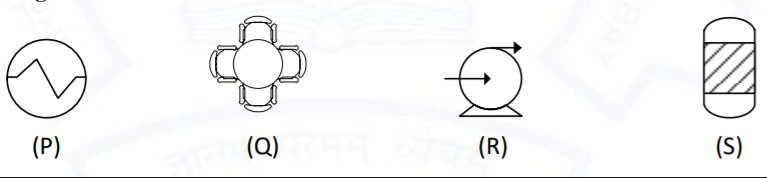
\includegraphics[width = 0.8\columnwidth]{q30all.png}
	\caption*{}
	\label{fig:a29ALL}
\end{figure}
\hfill{\brak{\text{GATE CH 2021}}}
\begin{enumerate}
	\begin{multicols}{2}
		\item (Q) and (S) only
		\item (P), (Q) and (R) only
		\item (P), (R) and (S) only
		\item (P), (Q), (R) and (S)
	\end{multicols}
\end{enumerate}

 

\item It is required to control the volume of the contents in the jacketed reactor shown in the figure.
\begin{figure}[H]
	\centering
	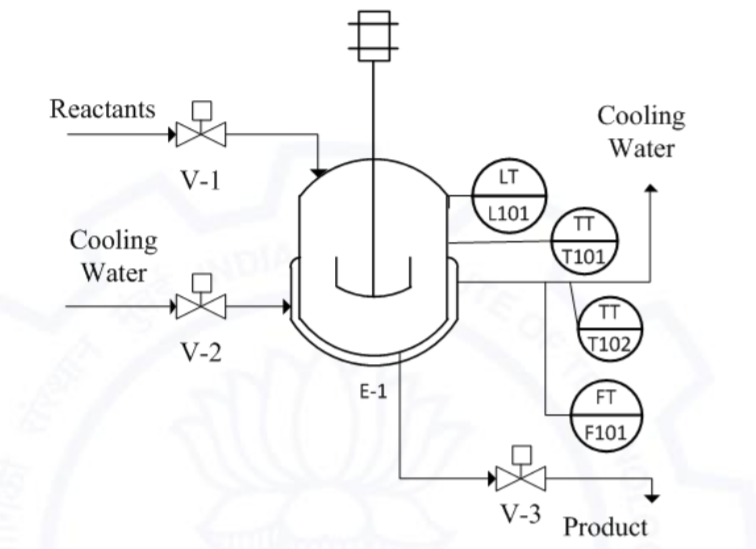
\includegraphics[width = 0.8\columnwidth]{q31.png}
	\caption*{}
	\label{fig:q31}
\end{figure}
Which one of the following schemes can be used for feedback control?
\hfill{\brak{\text{GATE CH 2021}}}
\begin{enumerate}
	\begin{multicols}{2}
		\item Measure L$101$ and manipulate valve V-$2$
		\item Measure T$101$ and manipulate valve V-$1$
		\item Measure L$101$ and manipulate valve V-$3$
		\item Measure F$101$ and manipulate valve V-$1$
	\end{multicols}
\end{enumerate}

 

\item Which of the following is NOT a necessary condition for a process under closed-loop control to be stable?
\hfill{\brak{\text{GATE CH 2021}}}
\begin{enumerate}
	\item Dead-time term(s) must be absent in the open-loop transfer function
	\item Roots of the characteristic equation must have negative real part
	\item All the elements in the left \brak{\text{first}} column of the Routh array must have the same sign
	\item Open-loop transfer function must have an amplitude ratio less than $1$ at the critical frequency
\end{enumerate}

 

\item Match the reaction in Group - 1 with the reaction type in Group - 2.
\begin{table}[H]
\centering
\begin{tabularx}{\textwidth}{|l|X|l|X|}
	\hline
	\multicolumn{2}{|c|}{Group - 1} & \multicolumn{2}{c|}{Group - 2} \\
	\hline
	P & Methylcyclohexane $\rightarrow$ Toluene + $3H_{2}$ & I & Dehydrocyclization \\
	\hline
	Q & Ethylcyclopentane $\rightarrow$ Methylcyclohexane & II & Cracking \\
	\hline
	R & n-Octane $\rightarrow$ Ethylbenzene + $4H_{2}$ & III & Dehydrogenation \\
	\hline
	S & n-Octane $\rightarrow$ n-Pentane + Propylene & IV & Isomerization \\
	\hline
\end{tabularx}
\caption*{}
\label{tab:q33}
\end{table}
The correct combination is:
\hfill{\brak{\text{GATE CH 2021}}}
\begin{enumerate}
\begin{multicols}{2}
	\item P-II, Q-III, R-I, S-IV
	\item P-III, Q-IV, R-I, S-II
	\item P-III, Q-IV, R-II, S-I
	\item P-I, Q-IV, R-III, S-II
\end{multicols}
\end{enumerate}

 

\item To solve an algebraic equation $f(x)=0$, an iterative scheme of the type $x_{n+1}=g(x_{n})$ is proposed, where $g(x)=x-\frac{f(x)}{f^{\prime}(x)}$. At the solution $x=s$, $g^{\prime}(s)=0$ and $g^{\prime\prime}(s)\ne0$. The order of convergence for this iterative scheme near the solution is \underline{\hspace{2cm}}.
\hfill{\brak{\text{GATE CH 2021}}}

 

\item The probability distribution function of a random variable X is shown in the following figure.
\begin{figure}[H]
\centering
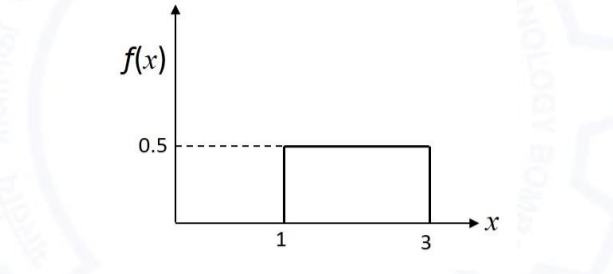
\includegraphics[width = 0.5\columnwidth]{q35.png}
\caption*{}
\label{fig:q35}
\end{figure}
From this distribution, random samples with sample size $n=68$ are taken. If $\overline{X}$ is the sample mean, the standard deviation of the probability distribution of $\overline{X},$ i.e. $\sigma_{\overline{X}}$ is \underline{\hspace{2cm}} \brak{\text{round off to 3 decimal places}}.
\hfill{\brak{\text{GATE CH 2021}}}

 

\item For the ordinary differential equation
\begin{align*}
\frac{d^{3}y}{dt^{3}}+6\frac{d^{2}y}{dt^{2}}+11\frac{dy}{dt}+6y=1
\end{align*}
with initial conditions $y\brak{0}=y^{\prime}\brak{0}=y^{\prime\prime}\brak{0}=0$, the value of $\lim_{t\rightarrow\infty}y\brak{t}$ is \underline{\hspace{2cm}} \brak{\text{round off to 3 decimal places}}.
\hfill{\brak{\text{GATE CH 2021}}}

 

\item Formaldehyde is produced by the oxidation of methane in a reactor. The following two parallel reactions occur.
\begin{align*}
CH_{4}+O_{2}&\longrightarrow HCHO+H_{2}O \\
CH_{4}+2O_{2}&\longrightarrow CO_{2}+2H_{2}O
\end{align*}
Methane and oxygen are fed to the reactor. The product gases leaving the reactor include methane, oxygen, formaldehyde, carbon dioxide and water vapor. $60$ mol $s^{-1}$ of methane enters the reactor. The molar flowrate \brak{\text{in mol } s^{-1}} of $CH_{4}$, $O_{2}$ and $CO_{2}$ leaving the reactor are $26$, $2$ and $4$, respectively. The molar flowrate of oxygen entering the reactor is \underline{\hspace{2cm}} mol $s^{-1}.$
\hfill{\brak{\text{GATE CH 2021}}}

 

\item The combustion of carbon monoxide is carried out in a closed, rigid and insulated vessel. $1$ mol of CO, $0.5$ mol of $O_{2}$ and $2$ mol of $N_{2}$ are taken initially at $1$ bar and $298$ K, and the combustion is carried out to completion. The standard molar internal energy change of reaction $\brak{\Delta u_{R}^{o}}$ for the combustion of carbon monoxide at $298$ K = $-282$ kJ $mol^{-1}$. At constant pressure, the molar heat capacities of $N_{2}$ and $CO_{2}$ are $33.314$ J $mol^{-1}$ $K^{-1}$ and $58.314$ J $mol^{-1}$ $K^{-1}$, respectively. Assume the heat capacities to be independent of temperature, and the gases are ideal. Take $R = 8.314~J~mol^{-1}K^{-1}$. The final pressure in the vessel at the completion of the reaction is \underline{\hspace{2cm}} bar \brak{\text{round off to 1 decimal place}}.
\hfill{\brak{\text{GATE CH 2021}}}

 

\item A gaseous mixture at $1$ bar and $300$ K consists of $20$ mol \% $CO_{2}$ and $80$ mol\% inert gas. Assume the gases to be ideal. Take $R=8.314~J~mol^{-1}K^{-1}$. The magnitude of minimum work required to separate $100$ mol of this mixture at $1$ bar and $300$ K into pure $CO_{2}$ and inert gas at the same temperature and pressure is \underline{\hspace{2cm}} kJ \brak{\text{round off to nearest integer}}.
\hfill{\brak{\text{GATE CH 2021}}}

 

\item Seawater is passed through a column containing a bed of resin beads.
\begin{tabularx}{\textwidth}{lX}
& Density of seawater $=1025~kg~m^{-3}$ \\
& Density of resin beads $=1330~kg~m^{-3}$ \\
& Diameter of resin beads $=50~\mu m$ \\
& Void fraction of the bed at the onset of fluidization $=0.4$ \\
& Acceleration due to gravity $=9.81~m~s^{-2}$ \\
\end{tabularx}
The pressure drop per unit length of the bed at the onset of fluidization is \underline{\hspace{2cm}} Pa $m^{-1}$ \brak{\text{round off to nearest integer}}.
\hfill{\brak{\text{GATE CH 2021}}}

 

\item A binary liquid mixture consists of two species $1$ and $2$. Let $\gamma$ and x represent the activity coefficient and the mole fraction of the species, respectively. Using a molar excess Gibbs free energy model, $\ln \gamma_{1}$ vs. $x_{1}$ and $\ln \gamma_{2}$ vs. $x_{1}$ are plotted. A tangent drawn to the $\ln \gamma_{1}$ vs. $x_{1}$ curve at a mole fraction of $x_{1}=0.2$ has a slope $=-1.728$. The slope of the tangent drawn to the $\ln \gamma_{2}$ vs. $x_{1}$ curve at the same mole fraction is \underline{\hspace{2cm}} \brak{\text{correct to 3 decimal places}}.
\hfill{\brak{\text{GATE CH 2021}}}

 

\item Consider a tank filled with $3$ immiscible liquids A, B and C at static equilibrium, as shown in the figure.
\begin{figure}[H]
\centering
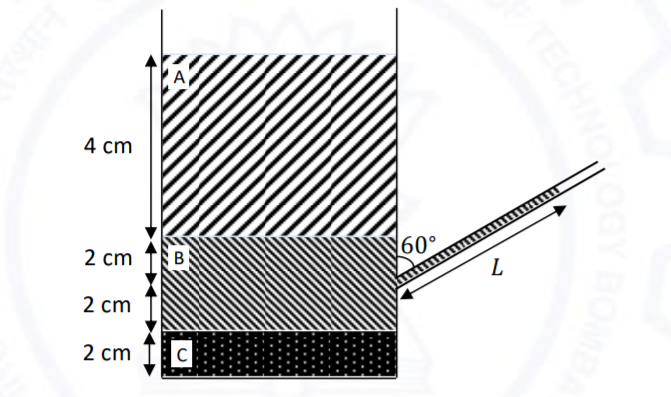
\includegraphics[width = 0.5\columnwidth]{q41.png}
\caption*{}
\label{fig:q42}
\end{figure}
At $2$ cm below the liquid A - liquid B interface, a tube is connected from the side of the tank. Both the tank and the tube are open to the atmosphere. At the operating temperature and pressure, the specific gravities of liquids A, B and C are $1$, $2$ and $4$, respectively. Neglect any surface tension effects in the calculations. The length of the tube L that is wetted by liquid B is \underline{\hspace{2cm}} cm.
\hfill{\brak{\text{GATE CH 2021}}}

 

\item A straight fin of uniform circular cross section and adiabatic tip has an aspect ratio \brak{\text{length/diameter}} of $4$. If the Biot number \brak{\text{based on radius of the fin as the characteristic length}} is $0.04$, the fin efficiency is \underline{\hspace{2cm}} \% \brak{\text{round off to nearest integer}}.
\hfill{\brak{\text{GATE CH 2021}}}

 

\item A double-effect evaporator is used to concentrate a solution. Steam is sent to the first effect at $110\degree C$ and the boiling point of the solution in the second effect is $63.3\degree C$. The overall heat transfer coefficient in the first effect and second effect are $2000$ W $m^{-2}K^{-1}$ and $1500$ W $m^{-2}K^{-1}$, respectively. The heat required to raise the temperature of the feed to the boiling point can be neglected. The heat flux in the two evaporators can be assumed to be equal. The temperature at which the solution boils in the first effect is \underline{\hspace{2cm}} $\degree C$ \brak{\text{round off to nearest integer}}.
\hfill{\brak{\text{GATE CH 2021}}}

 

\item Consider a solid slab of thickness $2L$ and uniform cross section A. The volumetric rate of heat generation within the slab is $\dot{g}\brak{Wm^{-3}}$. The slab loses heat by convection at both the ends to air with heat transfer coefficient h. Assuming steady state, one-dimensional heat transfer, the temperature profile within the slab along the thickness is given by:
\begin{align*}
T\brak{x} = \frac{\dot{g}}{2k}\brak{L^{2}-x^{2}}+T_{s} \text{ for } -L\le x\le L
\end{align*}
where k is the thermal conductivity of the slab and $T_{s}$ is the surface temperature. If $T_{s}=350~K$, ambient air temperature $T_{\infty}=300$ K, and Biot number \brak{\text{based on L as the characteristic length}} is $0.5$, the maximum temperature in the slab is \underline{\hspace{2cm}} K \brak{\text{round off to nearest integer}}.
\hfill{\brak{\text{GATE CH 2021}}}

 

\item A distillation column handling a binary mixture of A and B is operating at total reflux. It has two ideal stages including the reboiler. The mole fraction of the more volatile component in the residue $\brak{x_{w}}$ is $0.1$. The average relative volatility $\alpha_{AB}$ is $4$. The mole fraction of A in the distillate $\brak{x_{D}}$ is \underline{\hspace{2cm}} \brak{\text{round off to 2 decimal places}}.
\hfill{\brak{\text{GATE CH 2021}}}

 

\item In a batch drying experiment, a solid with a critical moisture content of $0.2$ kg $H_{2}O/kg$ dry solid is dried from an initial moisture content of $0.35$ kg $H_{2}O/kg$ dry solid to a final moisture content of $0.1$ kg $H_{2}O/kg$ dry solid in $5$ h. In the constant rate regime, the rate of drying is $2~kg~H_{2}O/\brak{m^{2}.h}$. The entire falling rate regime is assumed to be uniformly linear. The equilibrium moisture content is assumed to be zero. The mass of the dry solid per unit area is \underline{\hspace{2cm}} $kg/m^{2}$ \brak{\text{round off to nearest integer}}.
\hfill{\brak{\text{GATE CH 2021}}}

 

\item As shown in the figure below, air flows in parallel to a freshly painted solid surface of width $10$ m, along the z-direction.
\begin{figure}[H]
\centering
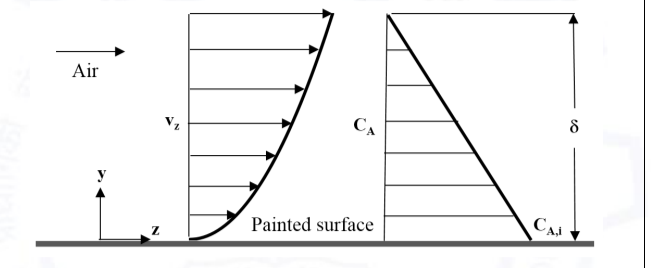
\includegraphics[width = 0.5\columnwidth]{q48.png}
\caption*{}
\label{fig:q48}
\end{figure}
The equilibrium vapor concentration of the volatile component A in the paint, at the air-paint interface, is $C_{A,i.}$ The concentration $C_{A}$ decreases linearly from this value to zero along the y-direction over a distance $\delta$ of $0.1$ m in the air phase. Over this distance, the average velocity of the air stream is $0.033$ m $s^{-1}$ and its velocity profile \brak{\text{in m } s^{-1}} is given by $v_{z}\brak{y}=10y^{2}$ where y is in meter. Let $C_{A,m}$ represent the flow averaged concentration. The ratio of $C_{A,m}$ to $C_{A,i}$, is \underline{\hspace{2cm}} \brak{\text{round off to 2 decimal places}}.
\hfill{\brak{\text{GATE CH 2021}}}

 

\item The following isothermal autocatalytic reaction,
\begin{align*}
A+B \xrightarrow{k_{1}} 2B
\end{align*}
is carried out in an ideal continuous stirred tank reactor \brak{\text{CSTR}} operating at steady state. Pure A at $1$ mol $L^{-1}$ is fed, and $90\%$ of A is converted in the CSTR. The space time of the CSTR is \underline{\hspace{2cm}} seconds.
\hfill{\brak{\text{GATE CH 2021}}}

 

\item Reactant A decomposes to products B and C in the presence of an enzyme in a well-stirred batch reactor. The kinetic rate expression is given by
\begin{align*}
-r_{A} = \frac{kC_{A}}{K_{M}+C_{A}}
\end{align*}
If the initial concentration of A is $0.02$ mol $L^{-1}$, the time taken to achieve $50\%$ conversion of A is \underline{\hspace{2cm}} min \brak{\text{round off to 2 decimal places}}.
\hfill{\brak{\text{GATE CH 2021}}}

 

\item The following homogeneous, irreversible reaction involving ideal gases,
\begin{align*}
A \rightarrow 2B + C
\end{align*}
is carried out in a steady state ideal plug flow reactor \brak{\text{PFR}} operating at isothermal and isobaric conditions. The feed stream consists of pure A, entering at $2$ m $s^{-1}$. In order to achieve $50\%$ conversion of A, the required length of the PFR is \underline{\hspace{2cm}} meter \brak{\text{round off to 2 decimal places}}.
\hfill{\brak{\text{GATE CH 2021}}}

 

\item A system has a transfer function $G(s) = \frac{10}{2s+1}$. When a step change of magnitude M is given to the system input, the final value of the system output is measured to be $120$. The value of M is \underline{\hspace{2cm}}.
\hfill{\brak{\text{GATE CH 2021}}}

 

\item A process has a transfer function $G(s) = \frac{Y(s)}{X(s)} = \frac{5\brak{-2s+1}}{10s+1}$. Initially the process is at steady state with $x \brak{t=0}=0.4$ and $y \brak{t=0}=100$. If a step change in x is given from $0.4$ to $0.5$, the maximum value of y that will be observed before it reaches the new steady state is \underline{\hspace{2cm}} \brak{\text{round off to 1 decimal place}}.
\hfill{\brak{\text{GATE CH 2021}}}

 

\item Operating labor requirements L in the chemical process industry is described in terms of the plant capacity C \brak{\text{kg day}^{-1}} over a wide range \brak{10^3-10^6} by a power law relationship $L = \alpha C^\beta$ where $\alpha$ and $\beta$ are constants. It is known that $L$ is $60$ when $C$ is $2 \times 10^4$ and $L$ is $70$ when $C$ is $6 \times 10^4$. The value of L when C is $10^5$ kg day$^{-1}$ is \underline{\hspace{2cm}} \brak{\text{round off to nearest integer}}.
\hfill{\brak{\text{GATE CH 2021}}}

 

\item A viscous liquid is pumped through a pipe network in a chemical plant. The annual pumping cost per unit length of pipe is given by $C_{pump} = 48.13 \frac{q^2\mu}{D^4}$. The annual cost of the installed piping system per unit length of pipe is given by $C_{piping} = 45.92D$. Here, D is the inner diameter of the pipe in meter, q is the volumetric flowrate of the liquid in m$^3$ s$^{-1}$ and $\mu$ is the viscosity of the liquid in Pa.s. If the viscosity of the liquid is $20 \times 10^{-3}$ Pa.s and the volumetric flow rate of the liquid is $10^{-4}$ m$^3$ s$^{-1}$, the economic inner diameter of the pipe is \underline{\hspace{2cm}} meter \brak{\text{round off to 3 decimal places}}.
\hfill{\brak{\text{GATE CH 2021}}}


\end{enumerate}
\end{document}